%%% 		cfp-m17n.tex :: mito / nyamcoder
\documentclass{article}
\usepackage[utf8]{mls} % alternativ: manjutex (veraltet)
\usepackage[encapsulated]{CJK} % notwendige Option!
\newcommand{\cjtext}[1]{\hspace{-2.5ex}\begin{CJK}{UTF8}{min}#1\end{CJK}} % für Japanisch + Hanzi
\usepackage{arabtex} % alternativ: arabi, auch für xelatex
\usepackage{kotex}  % \usepackage{hangul} fkt. hier wg. UTF-8 nicht!
\usepackage[svgnames]{xcolor}
\usepackage{pstricks-add,pst-grad,pst-text,pst-light3d,graphicx}
\makeatletter  % --->>> "interner LaTeX-Code": "@" wird normaler Buchstabe, lb2-16, 20, 875, 844
\def\placeChar#1{% %% für die gedrehte Platzierung der Kanji auf der Kreislinie; Dank an Herbert Voß für die Hilfestellung %%
\global\pst@cntm=162 % --> Winkelgrad, von wo die Platzierung beginnen soll
\expandafter\placeChar@i#1;}
\def\placeChar@i#1#2;{%  % ↓Kippwinkel ↓Angabe des Radius↓
\uput[\the\pst@cntm]{!180 \the\pst@cntm\space add}(5.4;\the\pst@cntm){\textbf{\large#1}}
\global\advance\pst@cntm by 5 % Schrittweite der Platzierung
\ifx\relax#2\relax\else\expandafter\placeChar@i#2;\fi}
\makeatother % <<<--- "@" wird wieder Sonderzeichen
\SetSansFonts{utgs}{utyt} % Änderung des Hanja-Fonts auf utyt ( 은 옛글, kotexguide.pdf, 39)
\pagestyle{empty}
\setlength\parindent{0ex}  % kein Einzug (Bild sonst zu nah am rechten Rand)
\begin{document}
%\vspace*{.3cm}\hspace*{-.5cm} % notwendige Verschiebung für komplette Anzeige von Gitter, Label und Mittelachse
%\psset{xunit=1cm,yunit=1cm,runit=1cm} % Standard-Einstellung für Länge von x-, y- und Radius-Einheit
\begin{pspicture}(0,0)(15,20)
\psframe[linewidth=.5pt,fillstyle=gradient,gradmidpoint=0,gradbegin=Honeydew,gradend=white](-3,-3)(15,23)
\rput(6,13.7){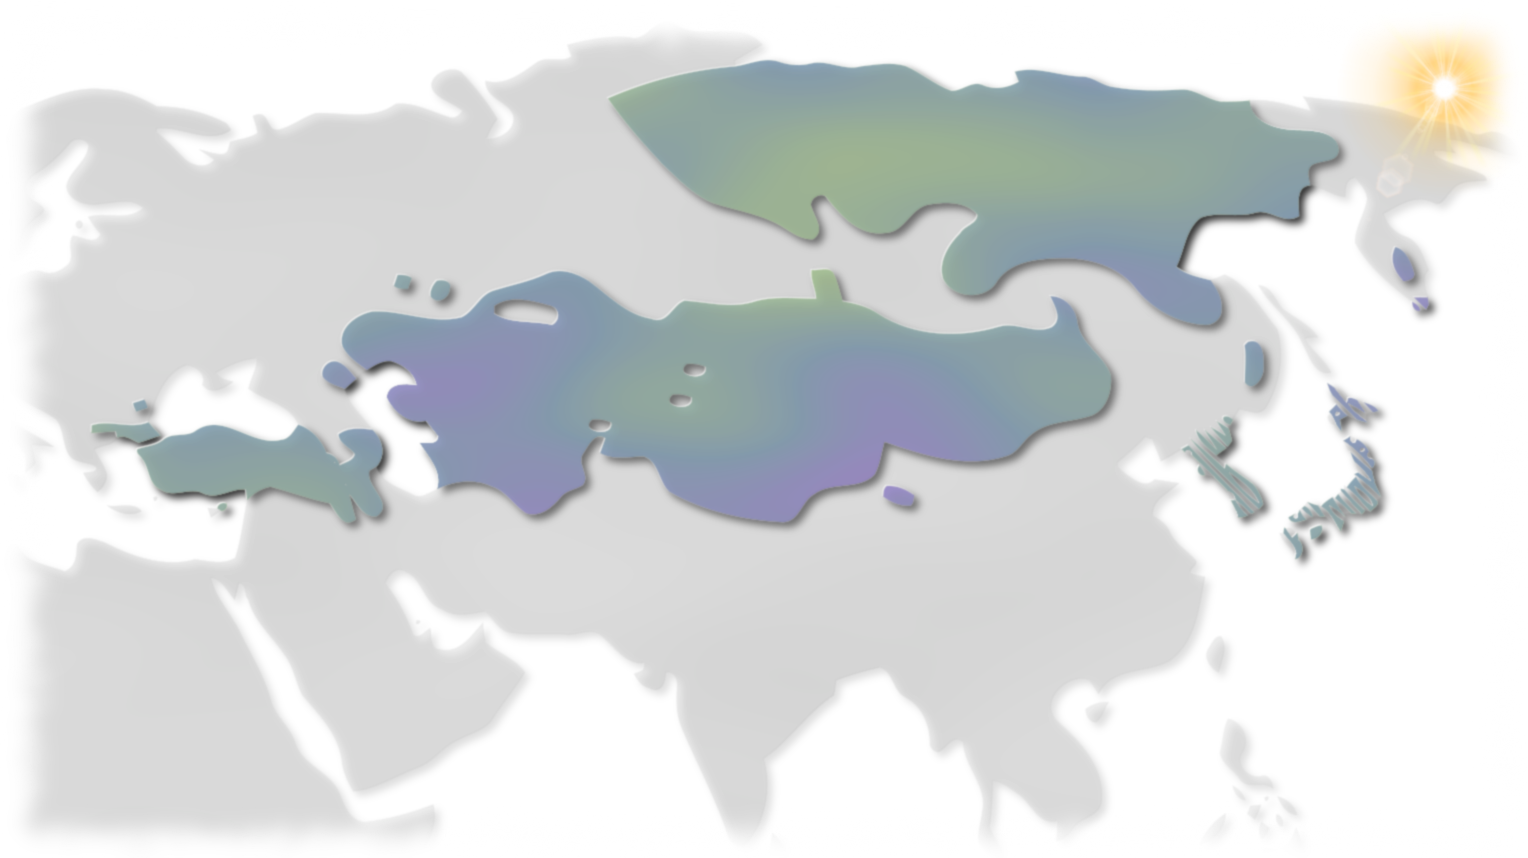
\includegraphics[width=12.4cm]{./pic/altailang-mito}}
\pstextpath[c]{
\psarcn[linestyle=none](6,13.7){5.7}{156}{354}}{
\color{DarkSlateBlue}{\large\textbf{• \xalx{\textit{Mongol utga zoxiol}} • {\fontsize{14}{16pt}\selectfont{한국문학}} • \textsf{Türk edebiyatı} • \bicig{munggul udg=a zukiyal}\enskip}}}
\pstextpath[l]{
\psarc[linestyle=none](6,13.7){5.7}{183}{214}}{
\color{DarkSlateBlue}{\large\bithe{manju s'u hvman}}}
\pstextpath[l]{
\psarc[linestyle=none](6,13.7){5.7}{214}{360}}{
\color{DarkSlateBlue}{\large\textbf{•\hspace{-.7ex}\cjtext{琉球文学} • \xalx{Bur\ya ad udxa zox"eol} • \hspace{-.5ex} {\fontshape{bf}\fontsize{14}{16pt}\selectfont{\setuighur\<uy^g\hspace{-.8ex}Nur :ad:abiyati>}} • \cjtext{蒙古文学} •}}}
% lat. Uy ur edebiyati; vgl. standardschreibung "uyghur" mit \<uy^gur ...> ƣ
\rput(6,13.8){
\color{DarkSlateBlue}{\placeChar{{{\cjtext{日}}}{{\cjtext{本}}}{{\cjtext{文}}}{{\cjtext{学}}}{{•}}}}}
\rput(6,17.9){\huge\color{Teal}\textbf{2010/8/12$\sim$17}}
\rput(6,9.6){\huge\color{Teal}\textbf{Seoul, Korea}}
\rput(9.8,13.2){\footnotesize\color{Crimson!80} •}  % Markierung für Seoul
\rput(6,21.2){\color{Teal}\textbf{\shortstack{제7 차 알타이어 언어학자, 작가,  번역가와 문예학자의 국제 회의\\
\scalebox{.9}[1]{\xalx{Alta"i sudlagq, utga zoxiogq, orqüülagq, utga zoxiolyn erdemtdi"in 7-r Olon Ulsyn Xural}}\\
\cjtext{第7 回 アルタイ諸語文学家・作家・翻訳家・評論家 国際会議}\\
\scalebox{.9}[1]{7. Enternasyonal Edebiyat Eleştirler, Yazarlar Tercümanlar ve Altay Dilbilimcilerin Konferans}\\[-.3ex]
7\raisebox{.5ex}{th} International Congress of Altaicists, Authors, Translators, and Literary Critics}}}
\rput(6,15.2){\PstLightThreeDText[linestyle=none,fillstyle=solid,fillcolor=Crimson!80,LightThreeDColorPsCommand=1.2 div 0.15 exch 0.7 exch sethsbcolor]{\fontsize{120}{120}\sffamily 鳳凰}}
\rput(6,14.2){\color{Teal}\sffamily\fontsize{30pt}{30pt}\selectfont 의}
\rput(6,13.2){\color{Khaki}\sffamily\fontsize{40pt}{50pt}\selectfont 歸還}
\rput(6,11.4){\huge\color{Crimson!80}\fontseries{bx}\shortstack{
\scalebox{.9}[1]{\xalx{\textit{Galt \sh uwuuny bucaj iräx n\i}}}\\[.5ex]
\sf\textbf{Anka Ku\c{s}unun Dönü\c{s}ü}\\[.35ex]
\fontshape{rm}\selectfont The\,Return\,of\,the\,Ph{\oe}nix}}
\rput(6,6.7){\color{Teal}\textbf{\shortstack{
\large  알타이어 문학의 전통과 유행\\
\xalx{\textit{Altayn\,töröl\,xälnüüdi"in\,utga\,zoxiolyn\,ulamjlalt\,ba"idal,\,sudlalyn\,\sh inä \,qigläl}}\\
\textsf{Altay dil ailesi edebiyatın eğilim ve gelenek}\\
Trends and Traditions in the Literature of the Altaic Languages}}}
\rput(6,5.45){\color{Crimson!80}CALL FOR PAPERS AND PARTICIPATION}
\rput(6,4.3){\color{Teal}\shortstack{\textsf{The Society of Altaic Literature and Music (SALM)} is pleased to announce the 7th International Congress\\of Altaicists, Authors and Literary Critics, 12-17 August, 2010, in Seoul, Korea.\\
Topics of interest include all kinds of literature produced\\
in the cultural and linguistic area of the Altaic language family, such as:}}
\rput(6,1.3){\color{DarkSlateBlue}\shortstack{
•  •  •  •  •  •  •  •  •  한글 몽골 위구르 터키 차가타이 만주 부랴트 일본 류큐 몽구오르 등의 다양한 문학\\
\textsf{Kore • Moğol • Türk • Çagatay • Mançurya • Uygur • Buryat • Ryukyu • Japonun daha çok edebiyatı}\\
Literature from the Korean • Khalkha • Oirat • Chakhar • Khorchin • Uighur • Turks •\\
Japanese • Manchu • Buryad • Ry\={u}ky\={u} • Monguor and many others . . .\\[1ex]
•  •  •  •  •  •  •  현대 문학 고전 문학 민간 설화 동화 소설 시정 전기 범죄 소설 등\\
\xalx{\textit{orcin cagi"in utga zoxiol • ardyn tuul\i{} • ülgäri"in oron • ögüülläg • roman • yaruu na"irag •}}\\
\xalx{\textit{namtar • gämt xärgi"in roman gäx mät}}\\
Modern fiction • classics • folk-tales • fairytales • short stories • novels • poetry •\\
biographies • crime novels etc.}}
\rput(6,-1.3){\color{Teal}\shortstack{Please submit a 200-word abstract by February 11, 2010, via e-mail to \textit{salcon@salm.or.kr}.\\
For more information about the conference please visit \textit{http://www.salm.or.kr/7thcon}.}}
% \psgrid[gridcolor=orange,gridlabelcolor=blue](0,0)(-4,-4)(16,24) % Hilfsgitter
% \psline[linecolor=blue](-4,0)(16,0) % x-Achse
% \psline[linecolor=blue](0,-4)(0,24) % y-Achse
% \psline[linecolor=red,linestyle=dashed,linewidth=2pt](6,-4.5)(6,24.5) % Mittelachse
\end{pspicture}
\end{document}


--> Bildquelle (./pic/altailang-mito, nachbearbeitet mit Gimp 2.6):
http://en.wikipedia.org/wiki/File:Altaic_family2.svg


--> Kompilation:
$ latex cfp-m17n && dvips cfp-m17n	&& ps2pdf cfp-m17n.ps
